% Options for packages loaded elsewhere
\PassOptionsToPackage{unicode}{hyperref}
\PassOptionsToPackage{hyphens}{url}
%
\documentclass[
  9pt,
]{article}
\usepackage{lmodern}
\usepackage{amssymb,amsmath}
\usepackage{ifxetex,ifluatex}
\ifnum 0\ifxetex 1\fi\ifluatex 1\fi=0 % if pdftex
  \usepackage[T1]{fontenc}
  \usepackage[utf8]{inputenc}
  \usepackage{textcomp} % provide euro and other symbols
\else % if luatex or xetex
  \usepackage{unicode-math}
  \defaultfontfeatures{Scale=MatchLowercase}
  \defaultfontfeatures[\rmfamily]{Ligatures=TeX,Scale=1}
\fi
% Use upquote if available, for straight quotes in verbatim environments
\IfFileExists{upquote.sty}{\usepackage{upquote}}{}
\IfFileExists{microtype.sty}{% use microtype if available
  \usepackage[]{microtype}
  \UseMicrotypeSet[protrusion]{basicmath} % disable protrusion for tt fonts
}{}
\makeatletter
\@ifundefined{KOMAClassName}{% if non-KOMA class
  \IfFileExists{parskip.sty}{%
    \usepackage{parskip}
  }{% else
    \setlength{\parindent}{0pt}
    \setlength{\parskip}{6pt plus 2pt minus 1pt}}
}{% if KOMA class
  \KOMAoptions{parskip=half}}
\makeatother
\usepackage{xcolor}
\IfFileExists{xurl.sty}{\usepackage{xurl}}{} % add URL line breaks if available
\IfFileExists{bookmark.sty}{\usepackage{bookmark}}{\usepackage{hyperref}}
\hypersetup{
  pdftitle={Quantiles},
  hidelinks,
  pdfcreator={LaTeX via pandoc}}
\urlstyle{same} % disable monospaced font for URLs
\usepackage[margin=1in]{geometry}
\usepackage{color}
\usepackage{fancyvrb}
\newcommand{\VerbBar}{|}
\newcommand{\VERB}{\Verb[commandchars=\\\{\}]}
\DefineVerbatimEnvironment{Highlighting}{Verbatim}{commandchars=\\\{\}}
% Add ',fontsize=\small' for more characters per line
\usepackage{framed}
\definecolor{shadecolor}{RGB}{248,248,248}
\newenvironment{Shaded}{\begin{snugshade}}{\end{snugshade}}
\newcommand{\AlertTok}[1]{\textcolor[rgb]{0.94,0.16,0.16}{#1}}
\newcommand{\AnnotationTok}[1]{\textcolor[rgb]{0.56,0.35,0.01}{\textbf{\textit{#1}}}}
\newcommand{\AttributeTok}[1]{\textcolor[rgb]{0.77,0.63,0.00}{#1}}
\newcommand{\BaseNTok}[1]{\textcolor[rgb]{0.00,0.00,0.81}{#1}}
\newcommand{\BuiltInTok}[1]{#1}
\newcommand{\CharTok}[1]{\textcolor[rgb]{0.31,0.60,0.02}{#1}}
\newcommand{\CommentTok}[1]{\textcolor[rgb]{0.56,0.35,0.01}{\textit{#1}}}
\newcommand{\CommentVarTok}[1]{\textcolor[rgb]{0.56,0.35,0.01}{\textbf{\textit{#1}}}}
\newcommand{\ConstantTok}[1]{\textcolor[rgb]{0.00,0.00,0.00}{#1}}
\newcommand{\ControlFlowTok}[1]{\textcolor[rgb]{0.13,0.29,0.53}{\textbf{#1}}}
\newcommand{\DataTypeTok}[1]{\textcolor[rgb]{0.13,0.29,0.53}{#1}}
\newcommand{\DecValTok}[1]{\textcolor[rgb]{0.00,0.00,0.81}{#1}}
\newcommand{\DocumentationTok}[1]{\textcolor[rgb]{0.56,0.35,0.01}{\textbf{\textit{#1}}}}
\newcommand{\ErrorTok}[1]{\textcolor[rgb]{0.64,0.00,0.00}{\textbf{#1}}}
\newcommand{\ExtensionTok}[1]{#1}
\newcommand{\FloatTok}[1]{\textcolor[rgb]{0.00,0.00,0.81}{#1}}
\newcommand{\FunctionTok}[1]{\textcolor[rgb]{0.00,0.00,0.00}{#1}}
\newcommand{\ImportTok}[1]{#1}
\newcommand{\InformationTok}[1]{\textcolor[rgb]{0.56,0.35,0.01}{\textbf{\textit{#1}}}}
\newcommand{\KeywordTok}[1]{\textcolor[rgb]{0.13,0.29,0.53}{\textbf{#1}}}
\newcommand{\NormalTok}[1]{#1}
\newcommand{\OperatorTok}[1]{\textcolor[rgb]{0.81,0.36,0.00}{\textbf{#1}}}
\newcommand{\OtherTok}[1]{\textcolor[rgb]{0.56,0.35,0.01}{#1}}
\newcommand{\PreprocessorTok}[1]{\textcolor[rgb]{0.56,0.35,0.01}{\textit{#1}}}
\newcommand{\RegionMarkerTok}[1]{#1}
\newcommand{\SpecialCharTok}[1]{\textcolor[rgb]{0.00,0.00,0.00}{#1}}
\newcommand{\SpecialStringTok}[1]{\textcolor[rgb]{0.31,0.60,0.02}{#1}}
\newcommand{\StringTok}[1]{\textcolor[rgb]{0.31,0.60,0.02}{#1}}
\newcommand{\VariableTok}[1]{\textcolor[rgb]{0.00,0.00,0.00}{#1}}
\newcommand{\VerbatimStringTok}[1]{\textcolor[rgb]{0.31,0.60,0.02}{#1}}
\newcommand{\WarningTok}[1]{\textcolor[rgb]{0.56,0.35,0.01}{\textbf{\textit{#1}}}}
\usepackage{graphicx}
\makeatletter
\def\maxwidth{\ifdim\Gin@nat@width>\linewidth\linewidth\else\Gin@nat@width\fi}
\def\maxheight{\ifdim\Gin@nat@height>\textheight\textheight\else\Gin@nat@height\fi}
\makeatother
% Scale images if necessary, so that they will not overflow the page
% margins by default, and it is still possible to overwrite the defaults
% using explicit options in \includegraphics[width, height, ...]{}
\setkeys{Gin}{width=\maxwidth,height=\maxheight,keepaspectratio}
% Set default figure placement to htbp
\makeatletter
\def\fps@figure{htbp}
\makeatother
\setlength{\emergencystretch}{3em} % prevent overfull lines
\providecommand{\tightlist}{%
  \setlength{\itemsep}{0pt}\setlength{\parskip}{0pt}}
\setcounter{secnumdepth}{5}
\usepackage{graphicx}
\usepackage{color}
\usepackage{hyperref}
\newcommand{\ve}[1]{\mathbf{#1}}
\newcommand{\sv}[1]{\boldsymbol{#1}}
\newcommand{\mat}[1]{\mathbf{#1}}
\newcommand{\sm}[1]{\boldsymbol{#1}}
\newcommand{\tr}[1]{{#1}^{\mkern-1.5mu\mathsf{T}}}
\newcommand{\norm}[1]{||{#1}||}
\newcommand{\given}{~\vline~}
\newcommand{\indep}{\bot\hspace{-.6em}\bot}
\newcommand{\notindep}{\bot\hspace{-.6em}\bot\hspace{-0.75em}/\hspace{.4em}}
\newcommand{\depend}{\Join}
\newcommand{\notdepend}{\Join\hspace{-0.9 em}/\hspace{.4em}}
\newcommand{\imply}{\Longrightarrow}
\newcommand{\notimply}{\Longrightarrow \hspace{-1.5em}/ \hspace{0.8em}}
\newcommand{\code}[1]{\texttt{#1}}
\newcommand*{\Rnsp}{\textsf{R}}
\newcommand*{\R}{\textsf{R}$~$}
\newcommand{\bigwig}[1]{\widetilde{#1}}

\title{Quantiles}
\author{}
\date{\vspace{-2.5em}}

\begin{document}
\maketitle

\begin{center}\rule{0.5\linewidth}{0.5pt}\end{center}

\textbf{29 marks}

\begin{enumerate}
\def\labelenumi{\arabic{enumi}.}
\item
  Suppose we have a continuous random variable \(X\) with distribution
  function \(F_X(x) = Pr(X \le x)\) and quantile function
  \(Q_X(p) = F_X^{-1}(p)\). That is \(p = F_X(x) = Pr(X \le x)\) and
  \(p = Pr(X \le Q_X(p)) = F_X(Q_X(p)) = F_X(F_X^{-1}(p)) = p\).

  \begin{enumerate}
  \def\labelenumii{\alph{enumii}.}
  \item
    \emph{(4 marks)} Suppose \(Y = aX +b\) for some constants \(a > 0\)
    and \(b\). \textbf{Prove} that a plot of the parametric curve
    \((Q_X(p), Q_Y(p))\) for \(p \in (0,1)\) must follow a straight
    line.

    Give the equation of that line. \[
     p = Pr(Y \le Q_Y(p)) = Pr(aX + b \le Q_Y(p) ) = F_X(\frac{Q_Y(p) - b}{a})\\
     P = F_X(Q_X(p))
     \]

    Therefore

    \[\frac{Q_Y(p)-b}{a} = Q_X(p)\\
     Q_Y(p) = aQ_X(p) + b
     \]
  \item
    \emph{(3 marks)} When \(F_X(x)\) and \(Q_X(p)\) are the cumulative
    distribution and quantile functions of the continuous random
    variable \(X\), show that if \(U \sim U(0,1)\), then

    \[Pr(Q_X(U) \le x )  = F_X(x). \] We have \(U \sim U(0,1)\) so that
    \(Pr(U < a) = a\) for \(a \in [0,1]\) therefore \[
     Pr(Q_X(U) \le x) = Pr(F_X(Q_X(U)) \le F_X(x)) \\
     = Pr(U \le F_X(x)) = F_X(x)
     \]
  \item
    The above result implies that we could generate \(n\) independently
    and identically distributed (i.i.d.) random realizations \(X\) from
    \(F_X(x)\) by generating \(n\) i.i.d. random realizations \(U\) from
    \(U(0,1)\) and defining \(X = Q_X(U)\).

    In \textsf{R}$~$ the function \texttt{runif()} will generate uniform
    pseudo-random numbers.

    (Similarly, \texttt{dunif()}, \texttt{punif()}, and \texttt{qunif()}
    will return the density, the distribution, and the quantile
    functions, respectively, for a uniform random variable. See
    \texttt{help("runif")} for details.

    \begin{enumerate}
    \def\labelenumiii{\roman{enumiii}.}
    \item
      \emph{(1 mark)} Write an \textsf{R}$~$ function

\begin{Shaded}
\begin{Highlighting}[]
\NormalTok{r\_unifgenFx <{-}}\StringTok{ }\ControlFlowTok{function}\NormalTok{(n, }\DataTypeTok{qfunction =}\NormalTok{ qnorm) \{}
                    \CommentTok{\# Insert your code here}
\NormalTok{                    random <{-}}\StringTok{ }\KeywordTok{runif}\NormalTok{(n)}
                    \KeywordTok{qfunction}\NormalTok{(random)}
\NormalTok{                     \}}
\end{Highlighting}
\end{Shaded}

      which will generate and return \texttt{n} pseudo random
      observations from the distrubution whose quantile function is the
      value of the argument \texttt{qfunction}. Show your code.
    \item
      \emph{(2 marks)} Execute the following code snippets to illustrate
      your code

\begin{Shaded}
\begin{Highlighting}[]
\CommentTok{\# make sure we all get the same result}
\KeywordTok{set.seed}\NormalTok{(}\DecValTok{1234567}\NormalTok{)}
\CommentTok{\# save the currentgraphical parameters and set \textasciigrave{}mfrow\textasciigrave{}}
\NormalTok{oldPar <{-}}\StringTok{ }\KeywordTok{par}\NormalTok{(}\DataTypeTok{mfrow =} \KeywordTok{c}\NormalTok{(}\DecValTok{1}\NormalTok{,}\DecValTok{2}\NormalTok{))}

\KeywordTok{hist}\NormalTok{(}\KeywordTok{r\_unifgenFx}\NormalTok{(}\DecValTok{1000}\NormalTok{),}\DataTypeTok{main =} \StringTok{"normal"}\NormalTok{, }\DataTypeTok{xlab=}\StringTok{"p"}\NormalTok{, }\DataTypeTok{col =} \StringTok{\textquotesingle{}maroon\textquotesingle{}}\NormalTok{, }\DataTypeTok{border=}\StringTok{"black"}\NormalTok{)  }\CommentTok{\# Standard normal}

\KeywordTok{hist}\NormalTok{(}\KeywordTok{r\_unifgenFx}\NormalTok{(}\DecValTok{1000}\NormalTok{, }\DataTypeTok{qfunction =}\NormalTok{ qunif), }\DataTypeTok{main =} \StringTok{\textquotesingle{}Uniform\textquotesingle{}}\NormalTok{, }\DataTypeTok{xlab =} \StringTok{\textquotesingle{}p\textquotesingle{}}\NormalTok{, }\DataTypeTok{col =} \StringTok{\textquotesingle{}green\textquotesingle{}}\NormalTok{,}\DataTypeTok{border=}\StringTok{"black"}\NormalTok{)}
\end{Highlighting}
\end{Shaded}

      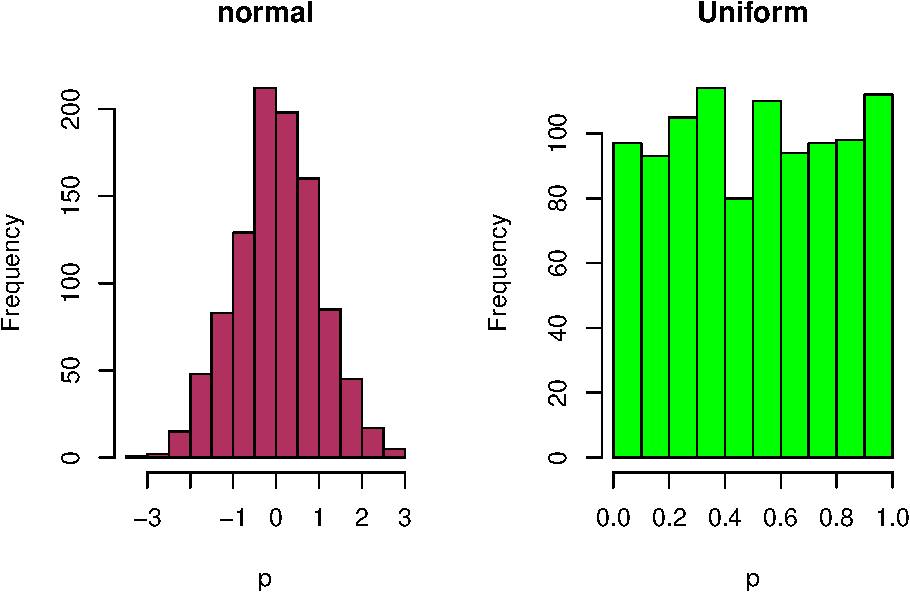
\includegraphics{quantiles_files/figure-latex/hists-1.pdf}

\begin{Shaded}
\begin{Highlighting}[]
\KeywordTok{par}\NormalTok{(oldPar) }\CommentTok{\# Return to original graphical parameters}
\end{Highlighting}
\end{Shaded}
    \item
      \emph{(2 marks)} Generate a sample of 1000 pseudo-random
      observations from a Student-t distribution on 3 degrees of freedom
      generated using \texttt{r\_unifgenFx()} (unchanged) and the
      quantile function of the Student-t. Plot a histogram
      (appropriately labelled) of the results.
    \end{enumerate}

\begin{verbatim}
   ```r
   set.seed(1234567)
   oldPar <- par(mfrow = c(1,2))
   hist(qt(r_unifgenFx(1000, qfunction = qunif), df=3), main = 'Student-t distribution', xlab = 'p', col = 'maroon')
   par(oldPar) # Return to original graphical parameters
   ```

   ![](quantiles_files/figure-latex/hist_t-1.pdf)<!-- --> 
\end{verbatim}
  \item
    Consider the \texttt{quantile()} function in \textsf{R}$~$.

    \begin{enumerate}
    \def\labelenumiii{\roman{enumiii}.}
    \tightlist
    \item
      \emph{(2 marks)} Explain the values returned by
      \texttt{quantile(mtcars\$qsec))}. That is, what does
      \texttt{quantile()} do? A quantile, or percentile, tells you how
      much of your data lies below a certain value.
    \end{enumerate}

\begin{Shaded}
\begin{Highlighting}[]
  \KeywordTok{quantile}\NormalTok{(mtcars}\OperatorTok{$}\NormalTok{qsec)}
\end{Highlighting}
\end{Shaded}

\begin{verbatim}
##      0%     25%     50%     75%    100% 
## 14.5000 16.8925 17.7100 18.9000 22.9000
\end{verbatim}

    For example, if we call quantile(mtcars\$qsec), it returns that the
    first 25\% values are in (14.5000, 16.8925), the second 25\% of the
    values are in (16.8925, 17.7100). The third 25\% values are in
    (17.7100, 18.9000) and the last 25\% values are in (18.9000,22.9000)

    \begin{enumerate}
    \def\labelenumiii{\roman{enumiii}.}
    \setcounter{enumiii}{1}
    \tightlist
    \item
      \emph{(2 marks)} Show how \texttt{quantile()} could be used to
      generate 1000 observations from the estimated distribution of
      \texttt{mtcars\$qsec}.
    \end{enumerate}
  \end{enumerate}
\end{enumerate}

\begin{Shaded}
\begin{Highlighting}[]
\NormalTok{  estimated\_qsec <{-}}\StringTok{ }\KeywordTok{quantile}\NormalTok{(mtcars}\OperatorTok{$}\NormalTok{qsec, }\DataTypeTok{probs =} \KeywordTok{runif}\NormalTok{(}\DecValTok{1000}\NormalTok{, }\DataTypeTok{min =} \DecValTok{0}\NormalTok{, }\DataTypeTok{max =}\DecValTok{1}\NormalTok{))}
\end{Highlighting}
\end{Shaded}

\begin{verbatim}
    iii. *(2 marks)* Would this work for `mtcars$cyl`? Why? Or, why not?
      No. The reason is the values if mtcars$cyl can be 4, 6, and 8 only. We cannot divide them into 4 quantiles.
    iv. *(4 marks)* Draw side by side (nicely labelled) histograms of `mtcars$qsec` and a sample of 1000 observations drawn from the estimated distribution of `mtcars$qsec`.  Comment on how these compare.
      
      ```r
      set.seed(1234567)
        oldPar <- par(mfrow = c(1,2))
        hist(mtcars$qsec,main = 'quarter-mile seconds', xlab = 'Seconds', col = 'yellow')
        hist(estimated_qsec, main = 'Estimated seconds', xlab = 'Seconds', col = 'maroon')
      ```
      
      ![](quantiles_files/figure-latex/unnamed-chunk-3-1.pdf)<!-- --> 
      
      ```r
        par(oldPar) 
      ```
      
      I think the estimation is very close to true.
    
    v. *(3 marks)* Draw a (nicely labelled) `qqplot()` comparing the above two sets of observations.  What do you conclude about their empirical distributions?  Why?
      
      ```r
        qqplot(mtcars$qsec, estimated_qsec, main = 'qqplot, quarter-mile seconds and estimated distribution', xlab = 'real qsec (s)', ylab = 'estimation(s)')
      ```
      
      ![](quantiles_files/figure-latex/unnamed-chunk-4-1.pdf)<!-- --> 
      The estimation is percise because the y-intercept of the plot is close to 0 and the slope is close to 1.

    vi. *(4 marks)* Suppose interest lay in producing a bootstrap distribution for some estimator $\bigwig{\theta}$.  Instead of bootstrapping, how might `quantile()` be used?  Which would you recommend and why?
      We can further use the quantile function for each 25% of the data. By making 4x4=16 quantiles, the result could be more close to th real data.
      Bootstraping is more complex and the result may depend on the representative sample.
\end{verbatim}

\end{document}
